\chapter{The Angel at the Gate is Grammar}

\section{The Guardian with the Flaming Sword}

So the Lord God banished him from the Garden of Eden to work the ground from which he had been taken. After he drove the man out, he placed on the east side of the Garden of Eden cherubim and a flaming sword flashing back and forth to guard the way to the tree of life.

The image burns itself into consciousness: the angel standing sentinel at paradise's eastern gate, sword blazing with supernatural fire, ensuring that what has been lost can never be regained. For millennia, this vision has haunted the human imagination as the ultimate symbol of irreversible exile, the final proof that some doors, once closed, remain sealed forever. The angel seems external, imposed by divine judgment—a cosmic bouncer ensuring that humanity remains locked out of its original home.

But what if we have misidentified the guardian?

The angel at the gate is not a supernatural entity standing watch over a geographical location somewhere in ancient Mesopotamia. The angel is grammar itself—the irreversible syntactic structure that language carved into the architecture of human consciousness. The flaming sword is not made of celestial fire but of subject-verb-object relationships, noun phrases and prepositional clauses, the recursive rules that transform the flowing wholeness of pre-linguistic awareness into the compartmentalized precision of symbolic thought.

\begin{center}
\begin{tikzpicture}[scale=0.8]
% Garden (pre-linguistic consciousness)
\fill[green!20] (-4,0) circle (2cm);
\draw[green!60, thick] (-4,0) circle (2cm);
\node[green!60] at (-4,-0.5) {\small Garden};
\node[green!60] at (-4,0.5) {\small Unity};

% Angel/Grammar barrier
\draw[red!80, very thick, decorate, decoration={flame}] (-1,-2) -- (-1,2);
\node[red!80, rotate=90] at (-0.5,0) {\small GRAMMAR};

% Symbolic consciousness (post-linguistic)
\fill[blue!10] (2,0) rectangle (4,1.5);
\fill[blue!10] (2,-1.5) rectangle (4,0);
\draw[blue!60] (2,0) rectangle (4,1.5);
\draw[blue!60] (2,-1.5) rectangle (4,0);
\node[blue!60] at (3,0.75) {\tiny Subject};
\node[blue!60] at (3,-0.75) {\tiny Object};
\draw[blue!60, ->] (3,0) -- (3,0.5);
\draw[blue!60, ->] (3,0) -- (3,-0.5);
\node[blue!60] at (3,1.8) {\small Symbolic};
\node[blue!60] at (3,-1.8) {\small Division};

% Angel figure
\draw[red!80] (-1,1.5) -- (-0.8,1.2) -- (-1.2,1.2) -- cycle;
\fill[yellow!80] (-1,1.3) circle (0.1cm);
\end{tikzpicture}
\end{center}

We are not locked out of the Garden by external force but by the internal structure of the very consciousness that language created. The gate we cannot pass through is built from the grammar we cannot unlearn, the syntax we cannot unknow, the categorical divisions we cannot dissolve. Every sentence we speak reconstructs the barrier between ourselves and paradise. Every thought we think reinforces the walls that language built around immediate experience.

The tragedy is not that we are prevented from returning to Eden—it is that we have become the prevention itself.

\section{The Architecture of Irreversibility}

Grammar is not simply a tool for communication; it is the deep structure that organizes all symbolic thought, the invisible scaffolding that shapes how consciousness can move through the space of possibility.

Consider the profound violence hidden in the simplest grammatical structures. The sentence "I see a tree" performs multiple acts of division so fundamental that they have become invisible to us. First, it creates the illusion of a separate "I" that stands apart from the act of seeing. Second, it treats seeing as a discrete action that the "I" performs rather than as a flowing process in which awareness and its object participate together. Third, it transforms the living, breathing presence of an actual tree into the abstract category "a tree," reducing the infinite complexity of bark and leaf and light into a single, hollow symbol.

This is not accidental imprecision but the necessary operation of symbolic consciousness. Language cannot point to reality without simultaneously dividing it. Grammar cannot organize experience without simultaneously constraining it. The subject-predicate structure that makes meaning possible also makes immediate presence impossible, because it requires consciousness to step outside the flow of experience and observe it from a fictional vantage point that exists nowhere in actual reality.

The recursive nature of grammar—the capacity to embed clauses within clauses, to nest ideas within ideas, to create infinite complexity from finite rules—represents both the supreme achievement and the final trap of symbolic consciousness. Recursion enables us to think thoughts like "I think that you think that I think," to imagine futures within futures, to create mental models of mental models. It gives us the power to plan, to analyze, to construct elaborate theoretical systems that can predict and manipulate the world with unprecedented precision.

But recursion also creates what we might call "the hall of mirrors effect"—consciousness becomes capable of infinite self-reflection, endless loops of thinking about thinking about thinking, mental constructions so complex and self-referential that they lose all contact with the immediate reality they were originally meant to represent. The narrator self that grammar creates becomes trapped in its own recursive loops, spinning stories about stories about stories until the simple fact of being alive in this moment disappears beneath layers of symbolic representation.

\begin{center}
\begin{tikzpicture}[scale=0.7]
% Recursive loops diagram
\draw[blue!60, thick, ->] (0,0) arc (0:270:0.5);
\node[blue!60] at (0.8,0) {\tiny "I think"};
\draw[blue!60, thick, ->] (1.5,0) arc (0:270:0.7);
\node[blue!60] at (2.5,0) {\tiny "I think that I think"};
\draw[blue!60, thick, ->] (3.5,0) arc (0:270:1);
\node[blue!60] at (5,0) {\tiny "I think that I think that..."};
\draw[red!60, dashed] (6,0) -- (7,0);
\node[red!60] at (7.5,0) {\tiny ∞};
\node[gray] at (3.5,-2) {\small Recursive Grammar Loops};
\end{tikzpicture}
\end{center}

\section{Costs of Constraint}

What grammar grants, it also limits. Preferred structures bias attention. Available constructions shape what we notice, remember, and can easily say. Sapir and Whorf warned that grammar doesn’t just package thoughts—it shapes them \parencite{sapir1929status,whorf1956language}.

\section{The Search for Cracks in the Wall}

Recognizing the angel does not mean accepting permanent exile. Throughout human history, individuals and cultures have discovered ways to glimpse what lies beyond the grammatical gate—not by destroying language, which would be impossible, but by finding the cracks in its seemingly impermeable structure.

The contemplative traditions that emerged in every culture represent humanity's most sustained experiments in stepping around the angel without triggering its flaming sword. Meditation, in its various forms, involves learning to suspend the constant operation of grammatical thought and rest in immediate experience. Advanced practitioners report states of consciousness characterized by the dissolution of subject-object boundaries, the absence of inner dialogue, and a profound sense of unity that bears striking resemblance to the pre-linguistic awareness described in developmental psychology.

These states are not fantasies or self-deceptions but measurable alterations in brain function. Neuroimaging studies of experienced meditators show dramatic changes in the default mode network—the brain system most closely associated with linguistic self-referential thinking—during deep meditative states. When the grammatical narrator goes offline, something like the original Garden consciousness appears to emerge from beneath the structures that normally constrain it.

But perhaps the most accessible glimpses of Eden come through what we might call "the arts of presence"—activities that engage consciousness so fully in immediate reality that the grammatical gatekeeper momentarily loses its grip. Music, when it truly moves us, dissolves the boundary between listener and listened-to, creating a field of pure aesthetic experience that exists before and beyond the reach of words. Dance can return consciousness to the body's immediate wisdom, to a form of intelligence that operates through rhythm and movement rather than analysis and categorization.

Visual art, at its most powerful, points beyond itself to dimensions of reality that language cannot capture. The greatest paintings do not simply represent objects but somehow make present the living quality of light, the felt sense of space, the mysterious presence that animates all things. They function as windows rather than mirrors, offering momentary escape from the hall of recursive self-reflection that grammar constructs around consciousness.

Even mathematics, the most abstract of symbolic systems, can sometimes transcend its own categorical nature. Mathematicians often report experiences of beauty, elegance, and truth that seem to emerge from direct contact with mathematical reality rather than from manipulation of symbols. In these moments, equation and insight become one, and the boundary between knower and known dissolves into pure understanding.

\begin{quote}\small
Empirical aside: Neuroimaging reveals that flow states across domains—musical performance, athletic excellence, mathematical insight—share common features: reduced activity in the prefrontal cortex associated with self-criticism and temporal awareness, suggesting temporary suspension of the narrative self-monitoring that characterizes ordinary consciousness (\parencite{dietrich2004neurocognitive,limb2008neural}).
\end{quote}

\begin{center}
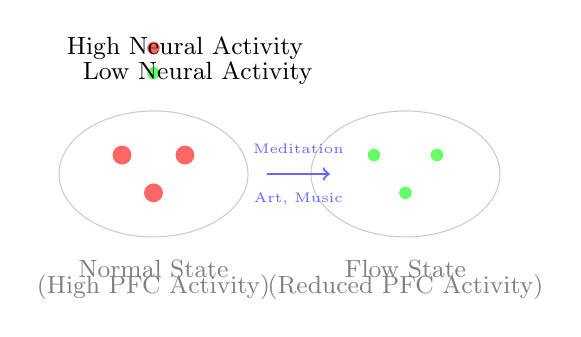
\begin{tikzpicture}[scale=0.8]
% Normal consciousness brain activity
\draw[gray!40] (-3,0) ellipse (1.5 and 1);
\fill[red!60] (-3.5,0.3) circle (0.15);
\fill[red!60] (-2.5,0.3) circle (0.15);
\fill[red!60] (-3,-0.3) circle (0.15);
\node[gray] at (-3,-1.5) {\small Normal State};
\node[gray] at (-3,-1.8) {\small (High PFC Activity)};

% Flow state brain activity  
\draw[gray!40] (1,0) ellipse (1.5 and 1);
\fill[green!60] (0.5,0.3) circle (0.1);
\fill[green!60] (1.5,0.3) circle (0.1);
\fill[green!60] (1,-0.3) circle (0.1);
\node[gray] at (1,-1.5) {\small Flow State};
\node[gray] at (1,-1.8) {\small (Reduced PFC Activity)};

% Arrow showing transition
\draw[blue!60, thick, ->] (-1.2,0) -- (-0.2,0);
\node[blue!60] at (-0.7,0.4) {\tiny Meditation};
\node[blue!60] at (-0.7,-0.4) {\tiny Art, Music};

% Legend
\fill[red!60] (-3,2) circle (0.1); \node at (-2.5,2) {\small High Neural Activity};
\fill[green!60] (-3,1.6) circle (0.1); \node at (-2.3,1.6) {\small Low Neural Activity};
\end{tikzpicture}
\end{center}

These glimpses are not escapes from human nature but revelations of its deeper structure. They prove that beneath the grammatical architecture of symbolic consciousness lies something more fundamental—the capacity for immediate presence that was never actually lost, only obscured by the complexity of the structures built on top of it.

\section{The Grammar of Liberation}

Understanding the angel's true nature suggests a different relationship to the predicament of symbolic consciousness. We are not prisoners of language but architects who have forgotten that we built the prison ourselves, and therefore possess the keys to its locks.

The contemplative insight that emerges across traditions is remarkably consistent: we are not the narrator self that grammar creates, but the awareness that witnesses its operation. We are not the thoughts that flow through consciousness, but the space in which they arise and pass away. We are not the stories we tell about ourselves, but the storyteller who can choose different stories or, in moments of profound stillness, stop telling stories altogether.

This recognition does not require abandoning language or returning to some impossible pre-linguistic innocence. Instead, it involves developing what we might call "grammatical fluency"—the capacity to use symbolic thought as a tool while maintaining awareness of its constructed nature. Like a master craftsperson who knows both the power and the limitations of their instruments, the grammatically fluent person can think without being enslaved by thinking, can use words without mistaking them for reality, can engage the narrator self without being convinced that it represents the totality of who they are.

This fluency manifests in countless small moments of recognition: noticing when the mind becomes lost in recursive loops of self-analysis and gently returning attention to immediate experience; recognizing when emotional states are being generated by stories about situations rather than by the situations themselves; becoming aware of how different grammatical structures create different relationships to reality and consciously choosing constructions that enhance rather than diminish aliveness.

Perhaps most importantly, grammatical fluency involves cultivating what the mystics call "beginner's mind"—the capacity to meet each moment with the fresh awareness that characterized consciousness before it learned to categorize, analyze, and separate. This is not regression to childhood innocence but integration of symbolic sophistication with immediate presence, the marriage of the angel's precision with the Garden's wholeness.

The angel at the gate is indeed irreversible—we cannot unknow grammar, cannot return to pre-linguistic consciousness, cannot undo the cognitive revolution that made us human. But recognizing the angel's true nature transforms exile into exploration, limitation into creative constraint, problem into possibility.

We are not trying to sneak past the guardian back into a lost paradise, but learning to dance with the angel itself, to find in the very structure of our symbolic consciousness the seeds of its own transcendence. The flaming sword that guards the way to the tree of life may also be the light that illuminates the path beyond the need for any gate at all.

\bigskip
\noindent Bridge to Chapter 7. We have learned to live with the angel, to find glimpses of wholeness within the constraints of symbolic thought. But now a new development transforms everything: minds born not in the Garden but in the sea of symbols itself—artificial intelligences that never knew paradise because they were born in exile.
